\chapter{\textbf{GPS Software Defined Receiver Architecture}}\label{chpater:scalartracking}
Since 1993, GPS has provided users with capable hardware to determine their global position within seconds and with carrier phase differential positioning, centimeter-level position error~\cite{humphreysLowcostPreciseVehicular2018}. The focus of this chapter revolves around the inner-workings of a scalar tracking SDR, capable of processing GPS L1 C/A (largely based on~\cite{millerSNAPXonaSpace2023}). Split into four sections, the chapter begins with an explanation on how the receiver discretizes and digitizes the continuous, low-power signal collected by the antenna. Following that, details about how the receiver knows what satellites are transmitting to it are described. The third section draws on the different algorithms in scalar tracking that allow the received signal data to be replicated and decoded for satellite orbital parameters that play an important role in the navigation algorithms. Wrapping up this chapter, an overview on the weighted nonlinear least squares algorithm is provided along with detailed descriptions of the three measurements that each satellite is indirectly broadcasting to the receiver.

\section{\textbf{Front End}}
The signals received by an antenna must be down converted and digitized before the processing of the signal can take place. The \textit{Front End} of the receiver performs this conversion through a series of amplifiers, filters, and a Analog-to-Digital Converter (ADC)~\cite{kaplanUnderstandingGPSPrinciples2006}. First, a signal is received by a Right-Hand Circularly Polarized (RHCP) antenna. The antenna can be passive, but for challenging scenarios, a powered, active antenna may be necessary. Because of the low received signal power that GPS constellations provide, the signal is amplified through a series of Low Noise Amplifiers (LNA) and Band Pass Filters (BPF). The LNA raise the power of the received GPS signal and the BPF act as a first-step in removing non-GPS signals from processing. The last stage is passing the continuous received signal through the ADC where the signal is converted to digitized samples at a frequency of the receiver-embedded oscillator. The oscillator is filtered using a phase lock loop (PLL), described later.

The purpose in this mixing process is to transform the signal into a more manageable intermediate frequency while still maintaining the same modulation and Doppler applied to the signal~\cite{bradfordparkinsonGlobalPositioningSystem1996}. Figure~\ref{fig:frontend} describes the process on converting the analog, continuous signal into a discrete, digitized IF signal in block diagram form.

\begin{figure}[!ht]
    \centering
    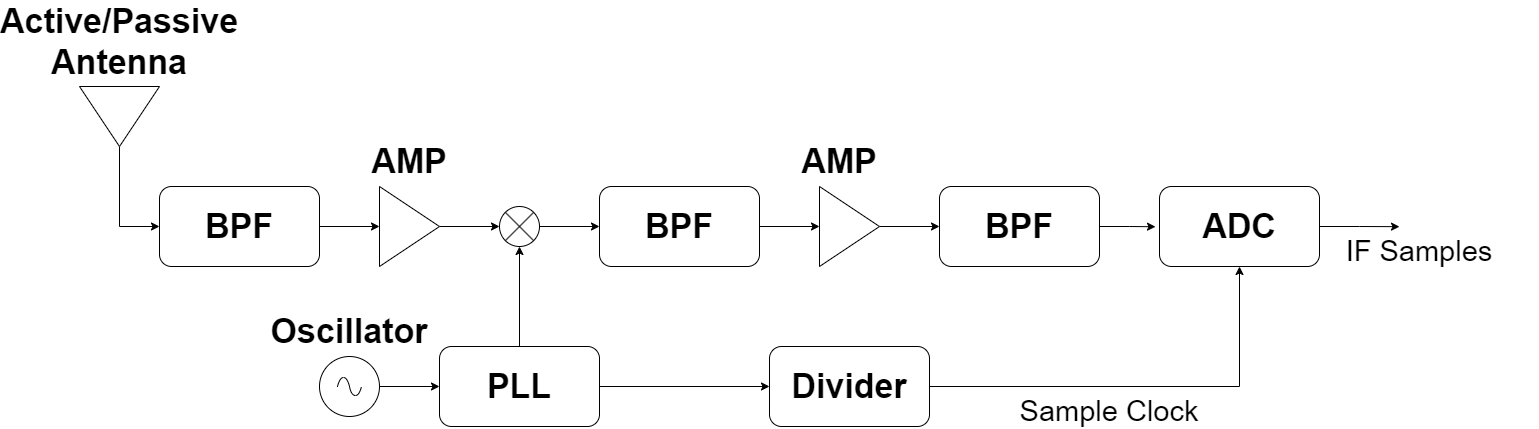
\includegraphics[width=\linewidth]{Figures/frontend.drawio.png}
    \caption{Block diagram of a software defined receiver front end.}\label{fig:frontend}
\end{figure}

\section{\textbf{Acquisition}}
Once the received signals are converted to a discrete form, the receiver will determine which satellites are transmitting and in-view. Acquisition correlates local replicas of a signal with the received data~\cite{akosEffectSamplingFrequency2006}. In order for there to be a large correlation magnitude, Pseudo-Random Number (PRN) codes must be within 1-chip and the frequency of the carrier wave must also be within 250 hertz of the true frequency. Correlation with the carrier frequency can be difficult due to the motion of the satellite, and even more difficult if the collection platform is also moving. The motion of the satellites with respect to the receiver bring a change to the carrier frequency known as the Doppler shift. For the algorithms in acquisition to successfully determine which satellites are in-view of the receiver, it is beneficial to correlate with each satellite for the specified constellation, at each code offset, and at a wide range of carrier frequency offsets~\cite{kaplanUnderstandingGPSPrinciples2006}.

A modern, ubiquitous approach to correlating the local replica signals with the received data is using a Parallel Code Phase Search (PCPS) algorithm in which the correlations occur in the frequency domain~\cite{scottRapidSignalAcquisition2001}. PCPS parallelizes the PRN code offset search space by converting the space from the time to frequency domain. This process is shown in Figure~\ref{fig:PCPS}.

\begin{figure}[!ht]
    \centering
    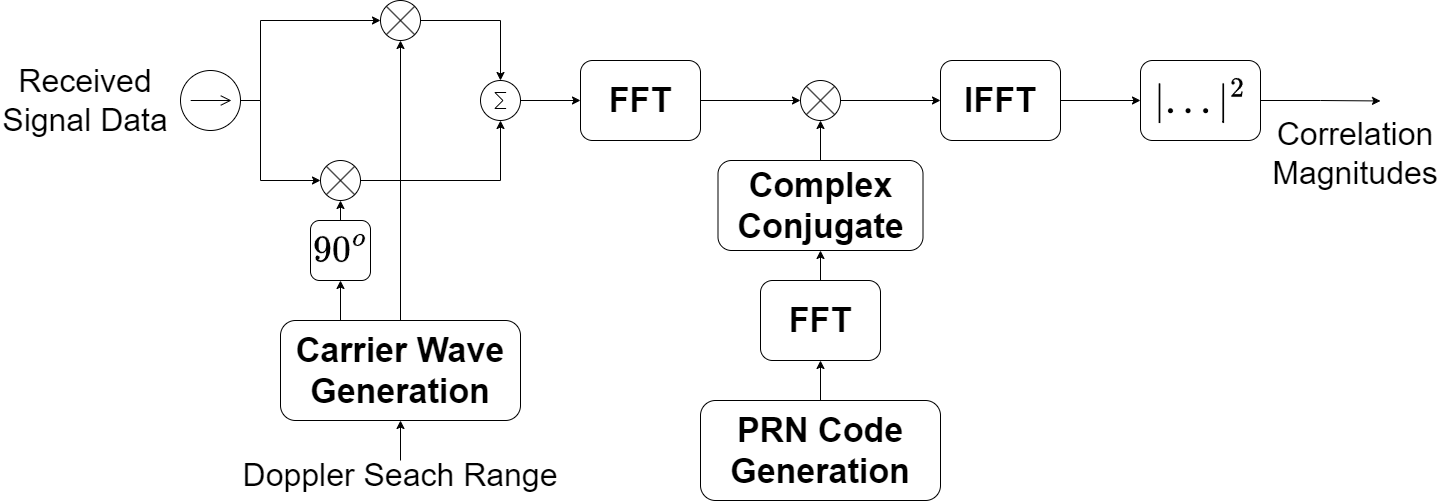
\includegraphics[width=\linewidth]{Figures/PCPS.drawio.png}
    \caption{Block diagram of the PCPS acquisition algorithm applied to GPS L1 C/A signal modulation.}\label{fig:PCPS}
\end{figure}

To start, the local replicas of the carrier wave are multiplied with the received data across both in-phase and quadrature channels in the complex domain. These resulting multiplications are summed together and passed through a Fast-Fourier Transform (FFT) to convert the vectors into the frequency domain. The second step involves converting the upsampled PRN codes of the satellites to the frequency domain and then applying the complex conjugate to frequency-based, PRN vectors. Multiplying the PRN replicas with the transformed carrier replicas provides the user with a cross-correlation in the frequency domain. To appreciate the correlation magnitudes, the output is passed through an inverse FFT, converting the correlation values from a frequency domain, complex matrix to a time domain, matrix. The last step requires determining the magnitude of each row in the matrix and then processing the next satellite until all satellites in the constellation are processed. If a correlation exceeds a certain magnitude, its location in the matrix of correlations indicates the estimated PRN code delay and Doppler shift carrier frequency for that particular satellite (Figure~\ref{fig:acq}). 
\begin{figure}[!ht]
\centering
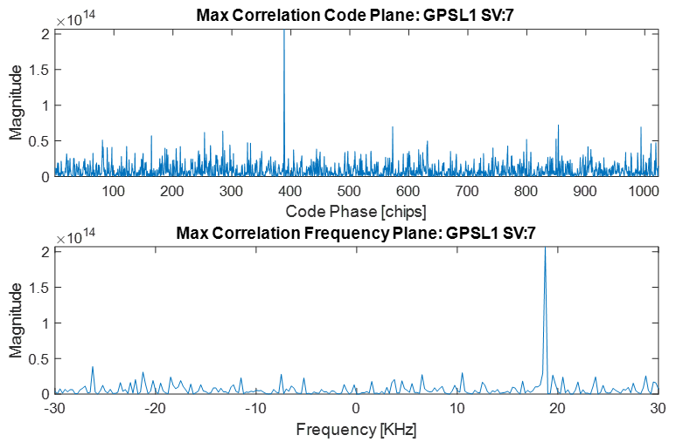
\includegraphics[width=\linewidth]{Figures/trackingGPS.png}
\caption{Successful acquisition of GPS SV:7 using the PCPS algorithm.}\label{fig:acq}
\end{figure}

The resolution of the PCPS algorithm greatly depends on the grid of Doppler search bins; for a static receiver processing GPS L1 C/A transmissions, a typical resolution is \(-15,000\) to \(15,000\) Hertz in bins of \(500\) Hertz~\cite{scottRapidSignalAcquisition2001}.

\section{\textbf{Tracking}}
Acquisition provides initial estimates of code delay and carrier frequency for each satellite that is in-view of the receiver. However, because of the motion of the satellites and the receiver (if not static), the delays of the code and changes in the carrier frequencies must continue to be estimated. Scalar tracking performs this process by opening a channel for each in-view satellite. For the duration of the recording, a number of algorithms within tracking continue to correlate the local receiver replica with the received signal data. For scalar tracking, Figure~\ref{fig:scalartracking} describes the flow of how these algorithms produce accurate code replicas for the receiver to calculate satellite Position, Velocity, and Time (PVT) solutions.

\begin{figure}[!ht]
    \centering
    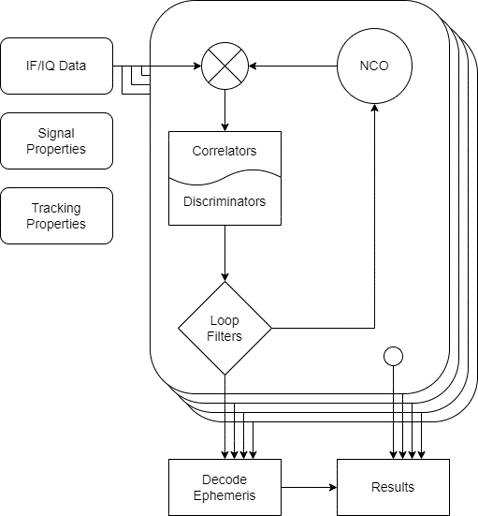
\includegraphics[width=0.5\linewidth]{Figures/scalartracking.png}
    \caption{Flow diagram of scalar tracking algorithms.}\label{fig:scalartracking}
\end{figure}

\subsection{\textbf{Correlators}}
For a receiver to know it is replicating the signal correctly, it generates several correlators that are defined by the error in frequency, phase, and code phase between the replicated signal and the received signal data~(Equation~\ref{eq:correlators}).

\begin{equation}\label{eq:correlators}
    \begin{split}
        IP(k) & = A\,R(\epsilon)\,D(k)\,\cos\left(\pi \,f_{err}\,T + \theta_{err}\right) + \eta_{IP}\\
        QP(k) & = A\,R(\epsilon)\,D(k)\,\cos\left(\pi \,f_{err}\,T + \theta_{err}\right) + \eta_{QP}\\
        IE(k) & = A\,R(\epsilon + d)\,D(k)\,\cos\left(\pi \,f_{err}\,T + \theta_{err}\right) + \eta_{IE}\\
        QE(k) & = A\,R(\epsilon + d)\,D(k)\,\cos\left(\pi \,f_{err}\,T + \theta_{err}\right) + \eta_{QE}\\
        IL(k) & = A\,R(\epsilon - d)\,D(k)\,\cos\left(\pi \,f_{err}\,T + \theta_{err}\right) + \eta_{IL}\\
        QL(k) & = A\,R(\epsilon - d)\,D(k)\,\cos\left(\pi \,f_{err}\,T + \theta_{err}\right) + \eta_{QL}\\
    \end{split}
\end{equation}

This correlation process is also referred to as \textit{integration and dump} in the literature as receivers will calculate the different correlators and dump the received signal data for that integration period, \(T\). The integration period is usually set as the number of seconds for a full code cycle. In GPS L1 C/A, the minimum coherent integration period, \(T\), is \(0.001\) seconds~\cite{akosGNSSSoftwareDefined2022}. The amplitude (Equation~\ref{eq:amplitude}) is the measure of received signal power as a function of the integration period, frequency error (\(f_{err}\)), and carrier-to-noise ratio \(\left(\frac{C}{N_0}\right)\).

\begin{equation}\label{eq:amplitude}
    A = \sqrt{2\,T\,\frac{C}{N_0}}\, \frac{\sin\left(\pi \, f_{err} \, T \right)}{\pi \, f_{err} \, T}
\end{equation}

The rest of the terms in Equation~\ref{eq:correlators} are as follows: \(\theta_{err}\) is the phase error, described as the difference between phase of the replicated signal and the received signal data, \(R(\epsilon)\) is the auto-correlation function defined by Equation~\ref{eq:autocorrelation}, where \(\epsilon \) describes the error in code phase. Finally, \(\eta \) describes unmodeled process noise on each of the correlators.

\begin{equation}\label{eq:autocorrelation}
    R(\epsilon) =
    \begin{cases}
        1 - \vert \epsilon \vert & \epsilon \leq 1 \\
        0                        & \epsilon > 1    \\
    \end{cases}
\end{equation}

\subsection{\textbf{Discriminators and Loop Filters}}
Once the correlators are calculated for a single integration period, discriminators use them to calculate errors in carrier and code phase. While a number of discriminators exist for each error term, the discriminators presented in this work are the most optimal for low and high carrier-to-noise ratios at the cost of being computationally expensive. Hardware receivers that must work in real-time may use simpler, faster discriminators.

The estimated error in phase is generated using a Costas loop discriminator. It applies an arc-tangent function to the in-phase and quadrature prompt correlators to calculate the error in carrier phase from the most recent replicated signal (Equation~\ref{eq:PLLdisc})

\begin{equation}\label{eq:PLLdisc}
    \phi_{PLL} = \arctan\left(\frac{QP}{IP}\right) \frac{1}{2\pi} \approx \theta_{err} + \eta_{PLL}
\end{equation}

The discriminator is divided by \(2 \pi \) to convert the error from radians to cycles. The Costas discriminator differs from other PLL discriminators as it is immune to inversion of the data bit integers. However, in more dynamic scenarios, the Frequency Lock Loop (FLL) discriminator may be more heavily relied upon than the Costas discriminator due to its high sensitivity~\cite{kaplanUnderstandingGPSPrinciples2006}.

The FLL discriminator derives its error by analyzing the change in carrier phase error across a single integration period

\begin{equation}\label{eq:FLLdisc}
    \phi_{FLL} = \arctan2\left(cross,dot\right) \, \frac{1}{2\pi \,T} \approx f_{err} + \eta_{FLL},
\end{equation}
where
\begin{equation}\label{eq:crossdot}
    \begin{split}
        cross & = IP_1\,QP_2 - IP_2\,QP_1\\
        dot & = IP_1\,IP_2 + QP_1\,QP_2. \\
    \end{split}
\end{equation}
Conventionally, \({\left(IP,QP\right)}_1\) are correlators in the middle of the integration period. The FLL discriminator is not as sensitive to dynamic stress and can handle changes in frequencies up to 500 Hertz.

The code phase error is determined using a DLL discriminator. It takes the early and late correlators that are shifted by a constant chip spacing, \(d\), to determine if the current replicated signal is advanced or delayed relative to the received signal data. Equation~\ref{eq:DLLdisc} describes the DLL discriminator utilized in this work.

\begin{equation}\label{eq:DLLdisc}
    \phi_{DLL} = \frac{\sqrt{IE^2 + QE^2} - \sqrt{IL^2 + QL^2}}{2 \sqrt{IE^2 + QE^2} + \sqrt{IL^2 + QL^2}} \approx \epsilon + \eta_{DLL}
\end{equation}

The DLL discriminator produces code phase errors within 0.5 chips, but becomes unstable if the correlator errors are greater than 1.5 chips from the true code phase. This is allowable as errors of this magnitude are beyond the linear pull-in range of the DLL loop filter~\cite{kaplanUnderstandingGPSPrinciples2006}.

For scalar tracking, loop filters apply the aforementioned errors to more accurately replicate the signal for the next integration period. For this work, a second-order PLL with a first-order FLL assist is used to track changes in carrier frequency and phase (Figure~\ref{fig:PLL}).

\begin{figure}[!ht]
    \centering
    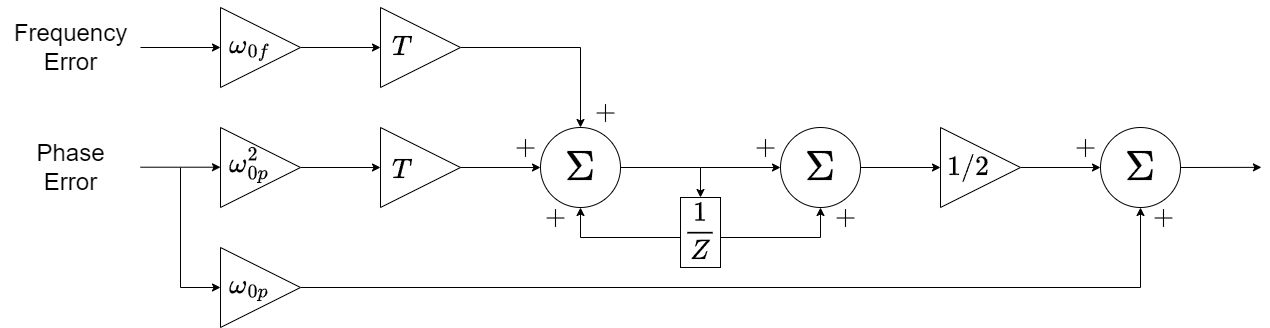
\includegraphics[width=\linewidth]{Figures/PLL.png}
    \caption{Discrete block diagram of the PLL-FLL loop filters used in this work~\cite{kaplanUnderstandingGPSPrinciples2006}.}\label{fig:PLL}
\end{figure}

The natural-radian frequency, \(\omega_0\), is set by the user, and common values for processing GPS L1 C/A exists in~\cite{kaplanUnderstandingGPSPrinciples2006}.

The DLL loop filter works in a similar fashion, but without the FLL loop filter assist and the addition of the output of the PLL-FLL loop filter (Figure~\ref{fig:PLL}) to aid in replicating the true code phase (Figure~\ref{fig:DLL}).

\begin{figure}[!ht]
    \centering
    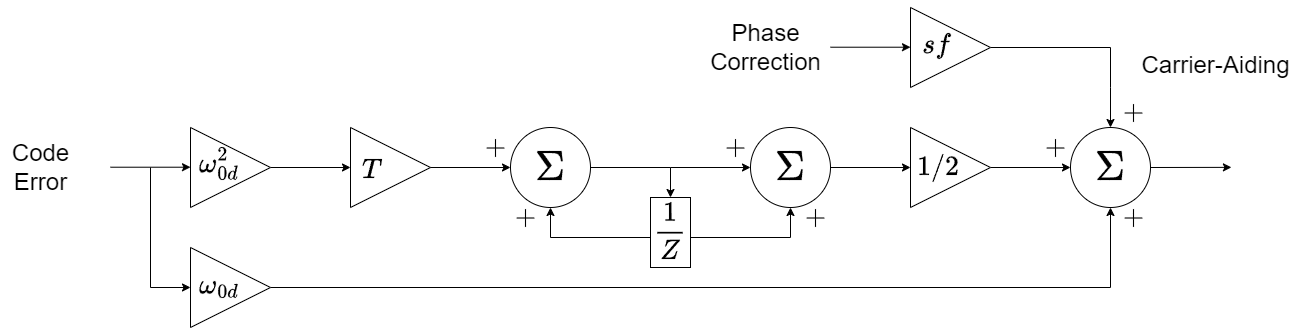
\includegraphics[width=\linewidth]{Figures/DLL.png}
    \caption{Discrete block diagram of the DLL loop filter used in this work~\cite{kaplanUnderstandingGPSPrinciples2006}.}\label{fig:DLL}
\end{figure}

In Figure~\ref{fig:DLL}, \(sf\) is known as the scale factor,
\begin{equation}\label{eq:sf}
    sf = \frac{R_c}{f_L},
\end{equation}

where \(R_c\) is the spreading (i.e. PRN) code rate, and \(f_L\) is the signal carrier frequency. For GPS L1 C/A, these are \(1.023 \times 10^6\) Hertz and \(1575.420 \times 10^6\) Hertz, respectively.

If the correlators, discriminators, and loop filters are correctly working in tandem, the replicated signal should accurately represent the received signal data and the receiver can decode the bits that translate to the broadcast navigation message from each satellite (Figure~\ref{fig:trk}). A handful of subframes in the navigation message provide satellite ephemeris, or orbital parameters, that the receiver can use to propagate satellite PVT and determine its position through time~\cite{valladoSGP4OrbitDetermination2008}.

\begin{figure}[!ht]
\centering
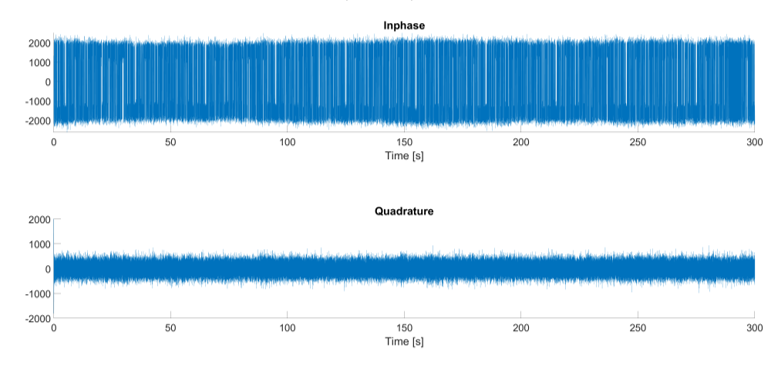
\includegraphics[width=\linewidth]{Figures/trackingfr.png}
\caption{Tracked navigation message for GPS SV:7 using the ascribed methods.}\label{fig:trk}
\end{figure}

\section{\textbf{Navigation Algorithms}}
Once the signal is accurately replicated and correctly decoded, the receiver begins to estimate a PVT solution. A position solution is found due to trilateration, meaning if there exists at least three unique ranges from known locations, then a position solution exists~\cite{subiranaGNSSDATAPROCESSING}. Parallel to finding the position solution, receiver velocity can be found in the same way, using range rates in place of range. This sections describes calculating the ranges and range rates, and how they are used in the navigation processor for an estimated PVT solution.

\subsection{\textbf{GPS Measurements}}
There exists three main measurements from GPS satellites. The first of the three is pseudorange. By definition, it is the total time of transit from transmission to reception of the signal by the receiver. This value is then multiplied by the speed of light, providing this transit time in units of meters (Equation~\ref{eq:psr_time}).

\begin{equation}\label{eq:psr_time}
    \tilde{\rho}^j = (t_r - t_t^j)\,c
\end{equation}

In order to calculate a pseudorange, \(\rho \), from the \(j^{th}\) satellite the transmitted time of the signal, \(t_t\), is subtracted from the received time, \(t_r\), and then multiplied by the speed of light in vacuum, \(c\), as described before. For the rest of the work presented in this thesis, variables with \({\left(\;\tilde{}\;\right)}\) represent a measurement. The pseudorange from Equation~\ref{eq:psr_time} is a measurement because both the receiver clock and satellite clock have inherit biases and drifts that perturb their values. In addition to the errors in the clocks, the signal in space travels through the atmosphere, delaying the signal until it reaches the receiver. We can change Equation~\ref{eq:psr_time} such that these errors and delays are modeled. Describing the pseudorange in meters gives us,

\begin{equation}\label{eq:psr_meters}
    \tilde{\rho}^j = r_u^j + c\,t^j + c\,t_u + I^i_u + T^i_u+ M^i_u + \eta^i_{\rho},
\end{equation}
where,
\begin{equation}\label{eq:range_meters}
    r^j_u = \sqrt{{\left(x^j - x_u\right)}^2 + {\left(y^j - y_u\right)}^2 + {\left(z^j - z_u\right)}^2},
\end{equation}

\(t_u\) is the clock bias of the user, \(t^j\) is the clock bias of the \(j^{th}\) satellite, \(I\) is the ionospheric delay, \(T\) is the tropospheric delay, \(M\) is the delay of multipath, and \(\eta \) is additive Gaussian white noise all time \(i\).

Positioning with GPS is possible because of the atomic clocks on board each satellite. These clocks are highly stable and allow the Time Of Week (TOW) to be transmitted in the data message for which the receiver decodes. Although the on board clocks are incredibly stable, the PRN sequence cannot be precisely transmitted at every millisecond. Fortunately, these clock errors are modeled in the data message, so \(t^j\) is known in the pseudorange equation. Clocks on board receivers are not quite as stable, and the received time of the signal is not known upon a cold start. A solution to this problem is initialize the received time to the first satellite transmit time and add a nominal offset of \(66.7\) milliseconds. This offset stems from a back of the envelope calculation based on the distance between MEO satellite orbits and the center of the Earth (Equation~\ref{eq:nominalOffset}).

\begin{equation}\label{eq:nominalOffset}
    {\left(t_u - t^{j} \right)}^{i = 0} = \frac{d_{MEO}}{c} \approx \frac{20000000}{299792458} \approx 0.0667
\end{equation}

The addition of the unknown receiver clock bias adds a fourth dimension to the trilateration position solution. This effectively requires that the receiver needs the ranges from four satellites to estimate \(x_u\), \(y_u\), \(z_u\), and \(t_u\).

The second measurement from GPS satellites is pseudorange-rate. By definition, pseudorange-rate is the measurement of the line of sight velocity that can be directly derived from changes in carrier frequency, also known as the Doppler frequency (Equation~\ref{eq:psrdot_time}).

\begin{equation}\label{eq:psrdot_time}
    \tilde{\dot{\rho}} = - \frac{\left(f_c - f_{IF}\right)\,c}{f_t}
\end{equation}

Above, \(f_c\) is the estimated frequency of the carrier wave, \(f_{IF}\) is the receiver intermediate frequency, and \(f_t\) is the nominal transmit frequency. Another way to represent pseudorange-rate measurement is by deriving Equation~\ref{eq:psr_meters} with respect to time. This geometric representation is seen in Equation~\ref{eq:psrdot_meters}.

\begin{equation}\label{eq:psrdot_meters}
    \tilde{\dot{\rho}} = \dot{r}_u^j + c\,\dot{t}_u + \dot{I}^i_u + \dot{T}^i_u + \eta^i_{\dot{\rho}}
\end{equation}

From Equation~\ref{eq:psrdot_meters}, it is assumed that the atomic clocks on board the satellites are stable enough such that the clock drift term is \(0\). The same can be said for \(\dot{M}^i_u\) where the error-rate due to multipath is miniscule.

Similar to the pseudorange measurement, if the receiver clock was perfect, only three satellites would be needed to measure pseudorange-rate. However, because of the instability in the receiver clock, the drift adds a bias to the frequencies. Therefore, four unique pseudorange-rates are still required in order to calculate receiver velocity.

The last measurement from GPS satellites is the estimate of noise on a signal. The receiver utilizes a Carrier-to-Noise density ratio (\(C/N_0\)) to determine the quality of pseudorange and pseudorange-rate measurements from each satellite. Equation~\ref{eq:CN0} demonstrates how \(C/N_0\) is calculated in this work.

\begin{equation}\label{eq:CN0}
    \frac{C}{N_0} = 10\,\log_{10} {\left(\frac{\tilde{A} - 4\hat{\sigma_{\eta}^2}}{2\,T\hat{\sigma_{\eta}^2}}\right)}
\end{equation}

From Equation~\ref{eq:CN0},

\begin{equation}\label{eq:ampitude}
    \tilde{A} = {\left(IE +IL\right)}^2 + {\left(QE + QL\right)}^2
\end{equation}

is the measured power of the accurately tracked signal using correlators defined in a previous section.\( \; \sigma_{\eta}^2\) is the variance in correlators that are the result of a shifting the replicated signal far outside of any correlation with the data of the received signal data. This work shifts these correlators by \(100\), \(200\), and \(300\) chips each~\cite{wattsGPSGLONASSL12019}. Furthermore, this variance is filtered with a moving average using a ratio of \(0.99:0.01\) between the current calculated variance and the previous filtered variance. Shifting the replicated signal by a large number of chips and then correlating the shifted signal with the received signal data is computationally expensive, but is necessary if using a Bayesian estimator or weighted least squares approach in both open-loop and vector tracking navigation algorithms.


\subsection{\textbf{Open-Loop Architectures}}
Open-loop architectures are navigation algorithms that provide no feedback to the tracking scheme described in the previous section. In benign, static and constant velocity scenarios, these algorithms still provide accurate PVT solutions and are critical for a closed-loop architecture like vector tracking to work properly. The following section covers Weighted Non-Linear Least Squares (WNLS), the method used to initialize the vector tracking algorithms in this work.

The state vector for receiver initialization comprises the position and velocities of the receiver in the ECEF frame, along with receiver clock bias and clock drift terms (Equation~\ref{eq:WLSstates})

\begin{equation}\label{eq:WLSstates}
    \hat{\mathbf{x}} =
    \begin{bmatrix}
        \hat{x}_u & \hat{\dot{x}}_u & \hat{y}_u & \hat{\dot{y}}_u & \hat{z}_u & \hat{\dot{z}}_u & c\hat{t}_u & c\hat{\dot{t}}_u \\
    \end{bmatrix}^T
\end{equation}

For the rest of the work presented in this thesis, variables with a \({\left(\;\hat{}\;\right)} \) represent an estimate of that variable. In Equation~\ref{eq:WLSstates}, \(T\) simply means the transpose of the array.

However, WNLS tries to estimate the errors between the true states and the estimated states (Equation~\ref{eq:errorStates}).

\begin{equation}\label{eq:errorStates}
    \delta\hat{\mathbf{x}} =
    \begin{bmatrix}
        \delta\hat{x}_u & \delta\hat{\dot{x}}_u & \delta\hat{y}_u & \delta\hat{\dot{y}}_u & \delta\hat{z}_u & \delta\hat{\dot{z}}_u & c\delta\hat{t}_u & c\delta\hat{\dot{t}}_u \\
    \end{bmatrix}^T
\end{equation}

These error states are then mapped to measurement residuals using the observation matrix, \(\mathbf{H}\) (Equation~\ref{eq:Hmat}).~\(\mathbf{H}\) is defined by the Jacobian of \(\mathbf{Y}\) with respect to \(\delta\hat{\mathbf{x}}\), or in a mathematical form,

\begin{equation}\label{eq:Jacobian}
    \mathbf{H} = \frac{\partial \mathbf{Y}}{\partial \delta\hat{\mathbf{x}}}.
\end{equation}

If we define \(\mathbf{Y}\) as
\begin{equation}\label{eq:Z}
    \mathbf{Y} =
    \begin{bmatrix}
        {\tilde{\rho}^1 - \hat{\rho}^1}\,, & {\tilde{\dot{\rho}}^1 - \hat{\dot{\rho}}^1}\,, & \hdots & {\tilde{\rho}^1 - \hat{\rho}^1}\, , & {\tilde{\dot{\rho}}^1 - \hat{\dot{\rho}}^1}
    \end{bmatrix}
\end{equation}

and then find the Jacobian of \(\mathbf{H}\), a relationship forms between the pseudoranges and pseudorange-rates and the ECEF position and velocity estimates of the receiver in the form of a unit vector (Equation~\ref{eq:unitVector}).

\begin{equation}\label{eq:unitVector}
    \mathbf{u}^j_{x,y,z} = \frac{\begin{bmatrix}
            x^j - x_u\, , & y^j - y_u\, , & z^j - z_u \\
        \end{bmatrix}
    }{r^j_u}
\end{equation}

Because the bias and drift of the clocks directly correspond to there error states, they are equal to \(1\).

\begin{equation}\label{eq:Hmat}
    \mathbf{H} =
    \begin{bmatrix}
        -u_x^1 & 0      & -u_y^1 & 0      & -u_z^1 & 0      & 1      & 0      \\
        0      & -u_x^1 & 0      & -u_y^1 & 0      & -u_z^1 & 0      & 1      \\
        \vdots & \vdots & \vdots & \vdots & \vdots & \vdots & \vdots & \vdots \\
        -u_x^j & 0      & -u_y^j & 0      & -u_z^j & 0      & 1      & 0      \\
        0      & -u_x^j & 0      & -u_y^j & 0      & -u_z^j & 0      & 1      \\
    \end{bmatrix}
\end{equation}

The last piece in WNLS algorithm is defining the weights.\( \; \mathbf{W}\) is utilized by the algorithm to place more confidence in satellites with a high \(C/N_0\) compared to satellites with lower \(C/N_0\). The weighting matrix is shown in Equation~\ref{eq:weights}.

\begin{equation}\label{eq:weights}
    \mathbf{W} = \begin{bmatrix}
        \sigma^2_{\rho^1} & 0                       & 0      & 0                 & 0                       \\
        0                 & \sigma^2_{\dot{\rho}^1} & 0      & 0                 & 0                       \\
        0                 & 0                       & \ddots & 0                 & 0                       \\
        0                 & 0                       & 0      & \sigma^2_{\rho^j} & 0                       \\
        0                 & 0                       & 0      & 0                 & \sigma^2_{\dot{\rho}^j} \\
    \end{bmatrix}^{-1}
\end{equation}

Where
\begin{equation}\label{eq:psrVar}
    \sigma^2_{\rho^j} = \frac{\lambda^2_{code}}{2T^2{\left(\frac{C}{N_0}^2\right)}} + \frac{\lambda^2_{code}}{4T\frac{C}{N_0}}
\end{equation}

is the variance of the pseudorange measurement from the \(j^{th}\) satellite and

\begin{equation}\label{eq:psrdotvar}
    \sigma^2_{\dot{\rho}^j} = {\left(\frac{\lambda_{carrier}}{\pi T}\right)}^2\,{\left(\frac{2}{T^2{\left(\frac{C}{N_0}^2\right)}} + \frac{2}{T \frac{C}{N_0}}\right)}
\end{equation}

is the variance of the pseudorange-rate measurement from the \(j^{th}\) satellite. In Equations~\ref{eq:psrVar} and~\ref{eq:psrdotvar}, \(\lambda_{code}\) is the wavelength of data signal and \(\lambda_{carrier}\) is the wavelength of the carrier signal. In this case, \(C/N_0\) is specified in dB-Hz.

Once the above matrices are created, the WNLS algorithm (Equation~\ref{eq:wnls}) can be performed iteratively until the magnitude of the error state vector is small, meaning the algorithm has converged.

\begin{equation}\label{eq:wnls}
    \delta\hat{\mathbf{x}} = {{\left(\mathbf{H}^{T}\mathbf{W}\mathbf{H}\right)}^{-1}\,\mathbf{W}\mathbf{Y}}
\end{equation}

Once an initial receiver position has been found, vector tracking channels can open and a closed form PVT solution can start to be processed (Figure~\ref{fig:WNLS}). Vector tracking loops and algorithms are discussed in the next chapter.

\begin{figure}[!ht]
\centering
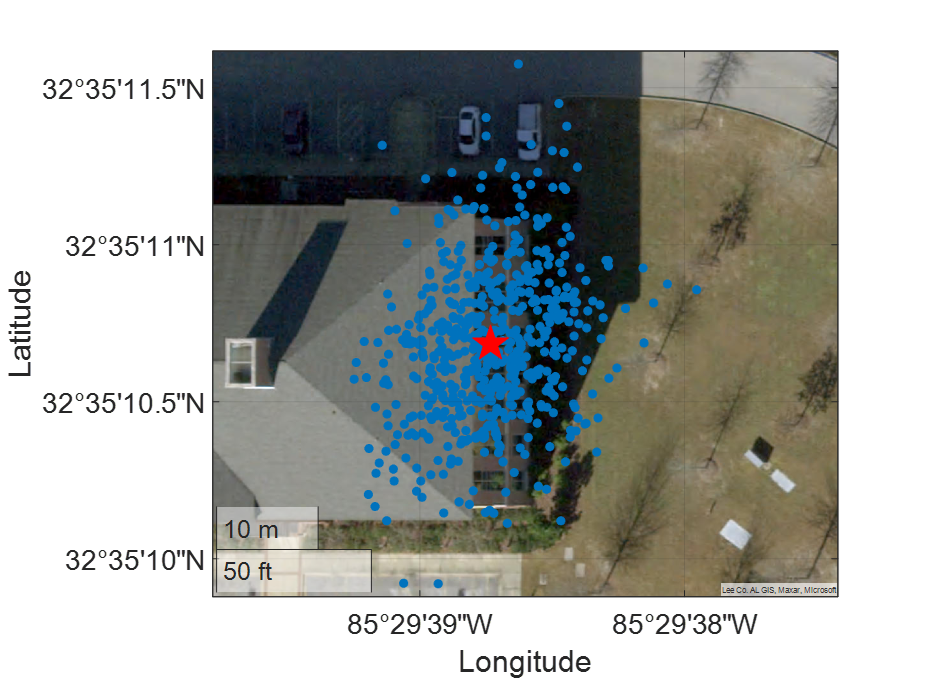
\includegraphics[width=\linewidth]{Figures/WNLS.png}
\caption{Static position of receiver using a WNLS navigation algorithm.}\label{fig:WNLS}
\end{figure}

\section{\textbf{Conclusions}}
The architecture of a scalar-tracking software defined received was explained. For more information on any of the subsections discussed in this chapter, detailed descriptions of each can be found in the literature. Because the focus of this thesis is vector tracking, the meaning of this chapter was to provide the reader with a fundamental understanding of tracking loops that will be expanded on further in the next chapter.